%
\documentclass[%
 reprint,
 amsmath,amssymb,
 aps,
]{revtex4-1}

\usepackage{graphicx}% Include figure files
\usepackage{dcolumn}% Align table columns on decimal point
\usepackage{bm}% bold math


\begin{document}
\begin{titlepage}
\begin{center}
\large{UNIVERSIDAD PRIVADA DE TACNA}\\
\vspace*{-0.025in}
\begin{figure}[htb]
\begin{center}

\includegraphics[width=8cm]{./Imagenes/upt}
\end{center}
\end{figure}
\vspace*{0.15in}
INGENIERIA DE SISTEMAS  \\

\vspace*{0.5in}
\begin{large}
TITULO:\\
\end{large}

\vspace*{0.1in}
\begin{Large}
\textbf{Trabajo-Encargado-N-05-SQL-y-NoSQL} \\
\end{Large}

\vspace*{0.3in}
\begin{Large}
\textbf{CURSO:} \\
\end{Large}

\vspace*{0.1in}
\begin{large}
BASE DE DATOS II\\
\end{large}

\vspace*{0.3in}
\begin{Large}
\textbf{DOCENTE(ING):} \\
\end{Large}

\vspace*{0.1in}
\begin{large}
 Patrick Cuadros Quiroga\\
\end{large}

\vspace*{0.2in}
\vspace*{0.1in}
\begin{large}
Integrantes: \\
\begin{flushleft}
Adnner Esperilla Ruiz		\hfill	(2015050543) \\

\vspace*{0.5in}
\begin{center}
2019-Tacna\\
\end{center}
\vspace*{2in}
\end{flushleft}
\end{large}
\end{center}

\end{titlepage}


\title{Comparación BD NoSQL}
\begin{abstract}
\begin{center}
\textbf{Resumen}
\end{center}

Se hara la comparacion de una base de datos NoSQL, dando a conocer sus caracteristicas principales y analiazando lo importante que son sus definiciones de los tipos de base de datos NoSQL con el fin de brindar conocimiento con que base de datos pueda trabajar segun sus repesctivas areas ,tambien veremos la creacion de base de datos , inserción y consultas de datos NoSQL mediante la plataforma Docker.\\

\textbf{Palabras clave:}   NoSQL,MySql, Docker.\\

\begin{center}
\textbf{Abstract}
\end{center}
The comparison of a NoSQL database will be done, making known its main characteristics, and analyzing what your NoSQL database will be in order to provide knowledge about the database in order to work with your reactive areas, we will also see the creation of the database, insertion and queries of NoSQL data through the Docker platform. \\

\end{abstract}



\maketitle

%\tableofcontents

\section {Introducción}\label{sec:1}

Ahora en nuestros tiempo que viene ser la era digital  el  manejo de la información se hace más complejo ya que la la cantidad de datos es abrumadora ;ya que por motivos mayores las personas busquen tecnologias que le ayuden a simplificar estos problemas  Las bases de datos relacionales son las mas comunes, pero en los últimos años ha aumentado el interés por las bases de datos NoSQL, que son un conjunto de tecnologias que ayudan el manejo de informacion y su distribucion segun la necesidad de las personas.
\par Entonces el presente documento hace un analisis y revision  de las tecnologías NoSQL, haciendo posible hacer una comparación facil de comprender ante cualquier usuario con conocimiento minimo en lo que es base de datos.\\

\par El resto de este articulo está organizado de la siguiente manera. En la Sección 2 se muestra los requisitos necesarios  y métodos usados para el desarrollo de este articulo. La Sección 3 se explican los resultados. Y finalmente, las conclusiones están en la Sección 4.



%-----------------------------------------------------------------
\section{Requisitos y Métodos}\label{sec:2}
\subsection{Materiales}
	\begin{itemize}
		\item Tener activado la virtualizacion en el Bios
		\item Para poder ejecutar contenedores Docker es necesario tener instalado Docker Community Edition (CE) en nuestro equipo
		\item Windows 10 64bit: Pro, Enterprise o Education, con al menos 4GB de RAM.
	\end{itemize}
\subsection{Métodos}
	\begin{itemize}
		\item Se utilizo como material artículos y libros relacionados a la base de datos NoSQL , repositorios ,paginas web.
	\end{itemize}
%-----------------------------------------------------------------
\section{Marco Teórico}\label{sec:3}
Una base de datos es un conjunto de datos pertenecientes a un mismo contexto y almacenados sistemáticamente para su posterior uso. En este sentido; una biblioteca puede considerarse una base de datos compuesta en su mayoría por documentos y textos impresos en papel e indexados para su consulta. Actualmente, y debido al desarrollo tecnológico de campos como la informática y la electrónica, la mayoría de las bases de datos están en formato digital, siendo este un componente electrónico, por tanto se ha desarrollado y se ofrece un amplio rango de soluciones al problema del almacenamiento de datos.Coniene las siguientes caracteristicas:
\begin{itemize}
	\item Se emplean métodos determinados para incluir datos nuevos y para borrar, modificar o recuperar los datos almacenados.
	\item Los datos son independientes de los programas que los usan.
	\item Los datos están interrelacionados, sin redundancias innecesarias.
\end{itemize}
\subsection{Tipos de base de datos}
	          \begin{itemize}
		\item Hay bases de datos relacionales, como MySQL, SQL Server y Oracle. Como su nombre lo indica utilizan el modelo relacional y siempre es mejor usarlas cuando los datos son consistentes y ya tienes algo planificado.
                     \item También existen las no relacionales, como MongoDB y Redis, conocidas como NO-SQL (Not Only SQL). Estas son más flexibles en cuanto a consistencia de datos y se han convertido en una opción que intenta solucionar algunas limitaciones que tiene el modelo relacional.
		\item Además hay otras BBDD no tan tradicionales, como las basadas en grafos o aquellas que tienen información cartográfica, que pueden servir, por ejemplo, si estás creando un e-commerce para encontrar relaciones entre los productos y las preferencias de los usuarios.
	           \end{itemize}
\subsection{Bases de datos relacional}
	          \begin{itemize}
		\item La interfaz estándar de programa de usuario y aplicación a una base de datos relacional es el lenguaje de consultas estructuradas (SQL)
                     \item Una base de datos relacional es un conjunto de tablas que contienen datos provistos en categorías predefinidas.
		\item Ejemplo modelo relacional:
                     \begin{center}
		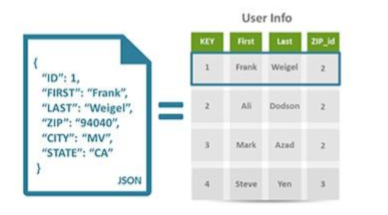
\includegraphics[width=9cm]{./Imagenes/1}
		\end{center}	
	          \end{itemize}
\subsection{Modelo NoSQL}
Las bases de datos NoSQL utilizan una variedad de modelos de datos para acceder y administrar datos, como documentos, gráficos, clave-valor, en-memoria y búsqueda. Estos tipos de bases de datos están optimizados específicamente para aplicaciones que requieren grandes volúmenes de datos, baja latencia y modelos de datos flexibles, lo que se logra mediante la flexibilización de algunas de las restricciones de coherencia de datos en otras bases de datos.\\\\
                     \begin{center}
		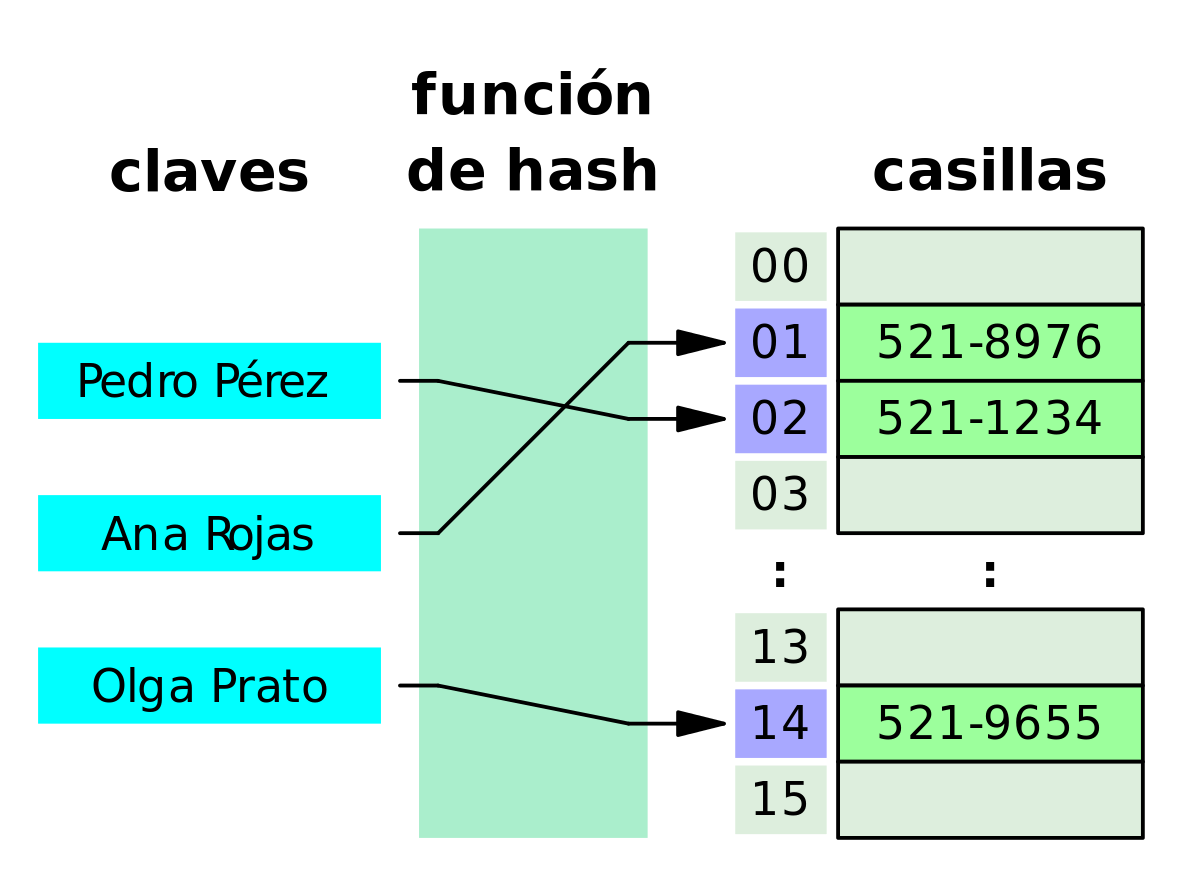
\includegraphics[width=8cm]{./Imagenes/2}
		\end{center}	
En una base de datos NoSQL, el registro de un libro generalmente se almacena como un documento JSON. Para cada libro, el elemento, ISBN, Título del libro, Número de edición, Nombre autor y IDAutor se almacenan como atributos en un solo documento. En este modelo, los datos están optimizados para un desarrollo intuitivo y escalabilidad horizontal.\\\\
as bases de datos NoSQL se adaptan perfectamente a muchas aplicaciones modernas, como dispositivos móviles, web y juegos, que requieren bases de datos flexibles, escalables, de alto rendimiento y altamente funcionales para proporcionar excelentes experiencias de usuario.\\\\
	           \begin{itemize}
		\item Flexibilidad:Las bases de datos NoSQL generalmente ofrecen esquemas flexibles que permiten un desarrollo más rápido y más iterativo. 
                     \item Escalabilidad: las bases de datos NoSQL generalmente están diseñadas para escalar usando clústeres distribuidos de hardware en lugar de escalar añadiendo servidores caros y sólidos. 
		\item Alto rendimiento:La base de datos NoSQL está optimizada para modelos de datos específicosy patrones de acceso que permiten un mayor rendimiento que el intento de lograr una funcionalidad similar con bases de datos relacionales.
		\item Altamente funcional:Las bases de datos NoSQL proporcionan API altamente funcionales y tipos de datos que están diseñados específicamente para cada uno de sus respectivos modelos de datos.
                     \begin{center}
		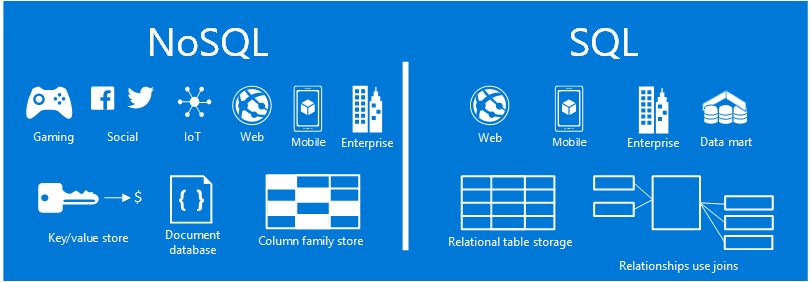
\includegraphics[width=8cm]{./Imagenes/3}
		\end{center}	
	          \end{itemize}
%-----------------------------------------------------------------
\section {Resultados}\label{sec:4}
\subsection{Creacion de base de datos NoSQL con MySql}
                     \begin{itemize}
		\item Mysql es una base NoSQL orientada a objetos
		\item Arquitectura cliente y servidor: MySQL, al igual que cualquier otro sistema de registros de datos, es un programa de registro basado en un sistema entre cliente y servidor.
		\item ompatibilidad con SQL: SQL es un lenguaje de programación que permite tanto la consulta como la renovación de datos para la gestión de una base en la que se almacena un conjunto de datos.
                     \item Lenguaje de programación: la base de datos MySQL está escrita en C y C++, dos de los lenguajes de programación más demandados y populares de todo el mundo.
                     \item Sistemas de almacenamiento: este tipo de bases proporciona sistemas de almacenamiento tanto transaccionales como no transaccionales.
                     \end{itemize}
\subsection{Instalar Mysql en Docker}
     \begin{itemize}
                     \item Ingresmos nuestra cuenta creada en Docker Hub para iniciar sesión en el aplicativo.Ubicar la aplicación PowerShell, ejecutarla como Administrador. En la ventana de comandos de PowerShell escribir lo siguiente:
                     \begin{center}
		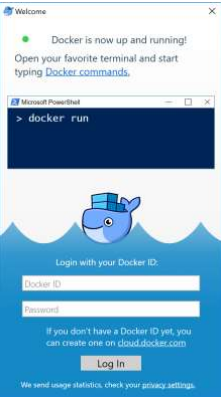
\includegraphics[width=5cm]{./Imagenes/8}
		\end{center}	
		\item Lo primero que hay que hacer es descargar el contenedor de Mysql con el siguiente comando.
                     \begin{center}
		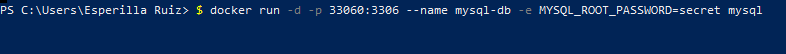
\includegraphics[width=8cm]{./Imagenes/14}
		\end{center}	
		\item Con esta tenemos nuestro contenedor escuchando
                     \begin{center}
		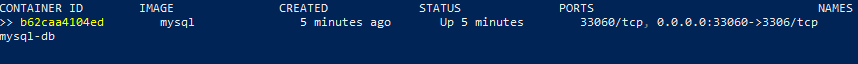
\includegraphics[width=10cm]{./Imagenes/9}
		\end{center}	
                     \item Para entrar al contenedor usamos un modo interactivo para asignar un TTY(terminal) y un STDIN abierto
                     \begin{center}
		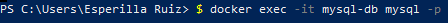
\includegraphics[width=8cm]{./Imagenes/15}
		\end{center}	
                     \begin{center}
		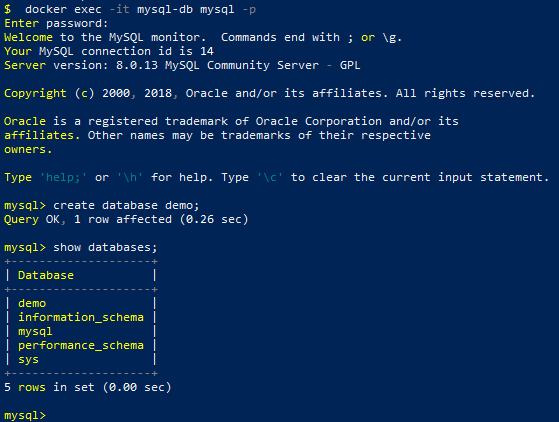
\includegraphics[width=8cm]{./Imagenes/16}
		\end{center}	
                     \item Eliminamos el proceso que corre el contenedor creado.
                     \begin{center}
		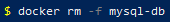
\includegraphics[width=3cm]{./Imagenes/17}
		\end{center}	
                     \item Eliminamos todos los volúmenes ya que Docker crea volúmenes temporales sin pedirte permiso.
                     \begin{center}
		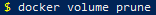
\includegraphics[width=3cm]{./Imagenes/18}
		\end{center}	
                     \item Creamos un volumen
                     \begin{center}
		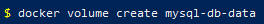
\includegraphics[width=3cm]{./Imagenes/20}
		\end{center}	
                    \item Verificamos que se haya creado el volumen
                     \begin{center}
		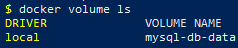
\includegraphics[width=5cm]{./Imagenes/21}
		\end{center}
                     \item Levantamos nuevamente el Docker y agregamos el volumen con la opcion --mount
                     \begin{center}
		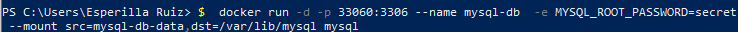
\includegraphics[width=7cm]{./Imagenes/22}
		\end{center}
                     \item Entramos al contenedor de forma interactiva o desde el Workbench y creamos una base de datos
                     \begin{center}
		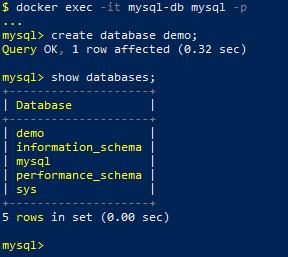
\includegraphics[width=8cm]{./Imagenes/23}
		\end{center}	
                      \item  Terminamos el proceso 
                     \begin{center}
		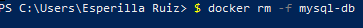
\includegraphics[width=7cm]{./Imagenes/24}
		\end{center}	                  
	          \end{itemize}
\subsection{Inserción y consulta de datos}
                     \begin{itemize}
		\item Inserccion de datos en la tabla  en MySql
                      \begin{center}
		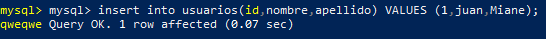
\includegraphics[width=8cm]{./Imagenes/26}
		\end{center}	
		\item Se hace copia el siguiente codigo para poder usar la consulta en Mysqli de una tabla 
                     \begin{center}
		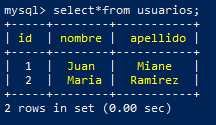
\includegraphics[width=5cm]{./Imagenes/27}
		\end{center}	
                  
	          \end{itemize}
\subsection{Comparación entre MySQL  y Oracle}
\textbf{MySQL}
\begin{itemize}
		\item MySQL es una fuente abierta y MySQL está disponible para su descarga e instalación gratuitas.
		\item La autenticación del usuario se realiza en MySQL usando solo la ubicación, el nombre de usuario y la contraseña.
		\item La flexibilidad de crear procedimientos y funciones almacenados utilizando PL / SQL es muy inferior en MySQL.
                     \item MySQL ofrece muy pocos comandos relacionados con la generación de resultados como informe y la definición de variables. MySQL incluye solo comandos SQL muy simples.
		\item MySQL no tiene la función de bóveda de auditoría en el servidor..
		\item MySQL no ofrece herramientas a nivel empresarial.
                     \item MySQL solo tiene facilidad de bloqueo de tablas.
		\item MySQL no tiene amplias funciones de almacenamiento como tablespace, sinónimo, paquetes y muchos otros.
		\item La base de datos MySQL no soporta XML.
                      \item MySQL solo admite dos tipos de caracteres, a saber, CHAR y VARCHAR.
		\item MySQL, las tablas temporales solo son visibles dentro de la sesión activa actual. Cuando la sesión expira, las tablas temporales se eliminan automáticamente.
		\item MySQL solo tiene dos mecanismos de copia de seguridad: mysqlhotcopy y mysqldump.
  \end{itemize}
\textbf{Oracle}
\begin{itemize}
		\item Solo Oracle Express Edition es gratuito. Pero Oracle Express Edition tiene características muy limitadas en comparación con MySQL
		\item Oracle proporciona seguridad de base de datos mejorada. La autenticación de usuarios se realiza en Oracle especificando roles globales además de la ubicación, el nombre de usuario y la contraseña
		\item Oracle proporciona funciones más flexibles para crear procedimientos y funciones almacenados utilizando PL / SQL.
                     \item Oracle incluye comandos SQL extensos en SQL * Plus, incluidos comandos para generar resultados como informe y definir variables.
		\item Oracle incluye comandos SQL extensos en SQL * Plus, incluidos comandos para generar resultados como informe y definir variables.
		\item Oracle proporciona instalaciones de bóveda de auditoría.
                     \item Oracle ofrece herramientas a nivel empresarial.
		\item Oracle proporciona la facilidad de bloqueo de fila también.
		\item Oracle tiene unas características de almacenamiento muy extensas. Oracle admite tablespace, sinónimo, paquetes y todas las demás características.
                      \item Oracle soporta y usa XML.
		\item Oracle admite cuatro tipos de datos de caracteres diferentes, a saber: CHAR, VARCHAR2, NCHAR, NVARCHAR2.
		\item Oracle ofrece muchos mecanismos de copia de seguridad, incluida la copia de seguridad en caliente, copia de seguridad, importación, exportación y muchos otros.
  \end{itemize}
\subsection{Documental}
Una base de datos documental, también llamada una base de datos orientada a documentos u tienda de documentos, es un subconjunto de un tipo de base de datos NoSQL.\\

Algunos almacenes de documentos también pueden ser bases de datos de valores clave. Una base de datos de documentos se utiliza para almacenar, recuperar y administrar datos semiestructurados.\\

A diferencia de las bases de datos relacionales tradicionales, el modelo de datos en una base de datos de documentos no está estructurado en un formato de tabla de filas y columnas.\\

El esquema puede variar, proporcionando mucha más flexibilidad para el modelado de datos que las bases de datos relacionales.\\

Las bases de datos documental almacena cada registro y sus datos asociados en un solo documento. Cada documento contiene datos semiestructurados que pueden ser consultados con el uso de varias herramientas de consulta y análisis del DBMS.
\begin{center}
	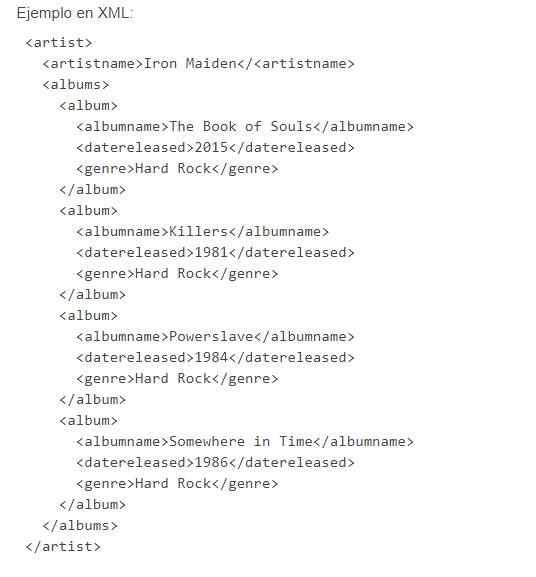
\includegraphics[width=8cm]{./Imagenes/documental1}
\end{center}	
.\\
\textbf{Fundamentos del formato JSON :}
\begin{itemize}
		\item Pares de valores clave o atributos :  Con el formato JSON se almacena en un par de valores clave. A estos pares se les llama a veces atributos. Las claves son cadenas simples y los valores pueden ser de cualquier tipo.
		\item Incrustación de objetos: Los valores incluidos en el par de valores clave también pueden ser otros objetos JSON, lo que permite crear una jerarquía de objetos. Colocar objetos JSON dentro de otro objeto JSON se denomina modelo de datos incrustados en base de datos documentales.
		\item Matrices: El formato JSON trabaja con un lenguaje de programación natural en todos los lenguajes de programación y estructuras de datos que son las matrices, por lo cual se admite almacenamiento de matrices como valores contra una clave. 
\end{itemize}
\begin{center}
	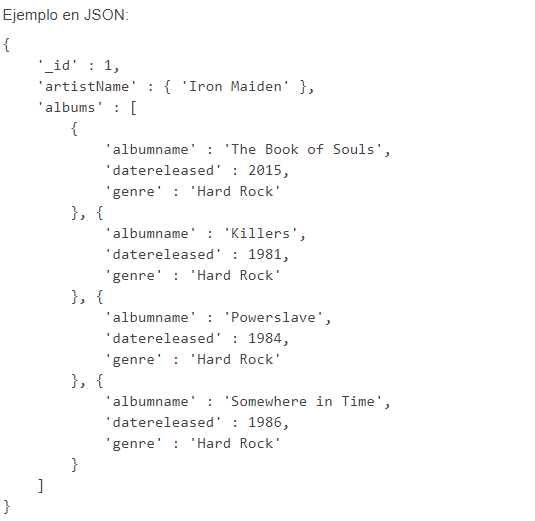
\includegraphics[width=9cm]{./Imagenes/documental2}
\end{center}	
En la imagen podemos ver un ejemplo de un documento de tipo JSON describe un libro.\cite{imagen}\\\\
\textbf{Beneficios :}
\begin{itemize}
		\item Modelado flexible de datos: a medida que las aplicaciones web, móviles, sociales e IoT cambian la naturaleza de los modelos de datos de aplicaciones, las bases de datos de documentos eliminan la necesidad de forzar modelos de datos relacionales para admitir nuevos tipos de modelos de datos de aplicaciones.
		\item Rendimiento de escritura rápido: a diferencia de las bases de datos relacionales tradicionales, algunas bases de datos de documentos priorizan la disponibilidad de escritura sobre la estricta consistencia de los datos. Esto garantiza que las escrituras siempre serán rápidas, incluso si una falla en una parte del hardware o de la red da como resultado un pequeño retraso en la replicación de datos y la coherencia en todo el entorno.
		\item Rendimiento rápido de consultas: muchas bases de datos de documentos tienen potentes motores de búsqueda y funciones de indexación que proporcionan capacidades de consulta rápidas y eficientes.
\end{itemize}
\subsection{Clave-Valor}
\begin{itemize}

                     \item Una base de datos clave-valor es un tipo de base de datos no relacional que utiliza un método simple de clave-valor para almacenar datos. Una base de datos clave-valor almacena datos como un conjunto de pares clave-valor en los que una clave sirve como un identificador único.
                     \begin{center}
		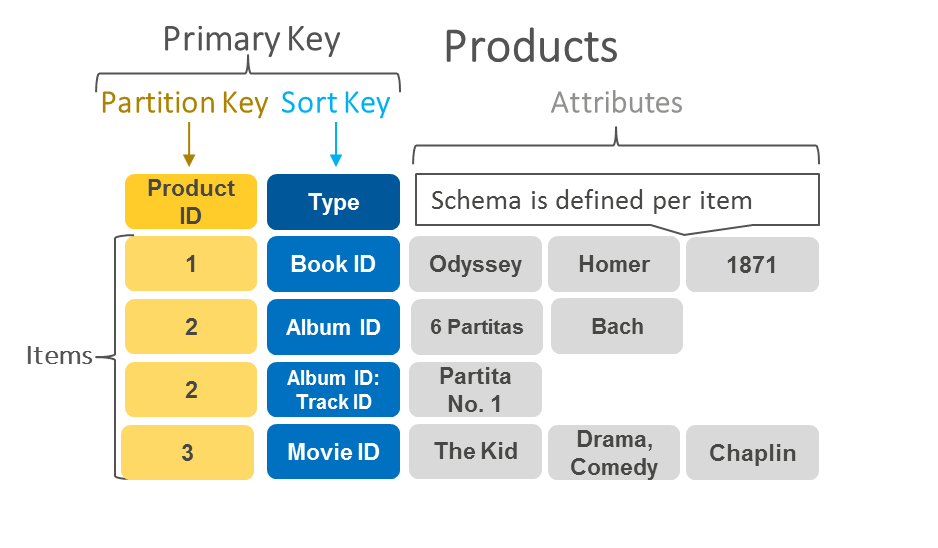
\includegraphics[width=6cm]{./Imagenes/30}
		\end{center}	
	          \end{itemize}

\subsection{Grafos}
\begin{itemize}
		\item En nuestras base de datos se puede utilizar el modelo de Grafos para ayudar .
		\item Disponer de más información con agilidad y eficiencia
		\item Las podemos utilizar por ejemplo para guardar puntos de un camino, relaciones de amigos, familia, o cualquier tipo de  dato que represente alguna relación
                     \item Consultas más amplias y no demarcadas por tablas
                     \begin{center}
		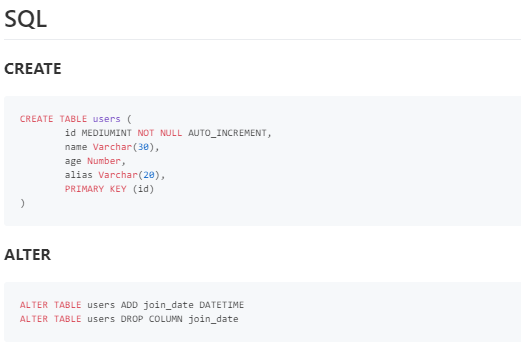
\includegraphics[width=8cm]{./Imagenes/4}
		\end{center}	
	          \end{itemize}
.
\subsection{Tabular (Column-Store)}
\begin{itemize}
		\item Las ventajas de rendimiento en los índices de almacén de columnas son posibles al aprovechar la tecnología de compresión VertiPaq, que permite que grandes cantidades de datos se compriman en la memoria.
		\item Lo datos son almacenados en columnas.
		\item En una columna tiene múltiples datos.
                     \item Un índice de almacén de columnas es más eficiente para este ejemplo porque solo se necesita una página de datos (comprimidos) de menor tamaño para satisfacer la consulta.
	          \end{itemize} 
 \begin{center}
	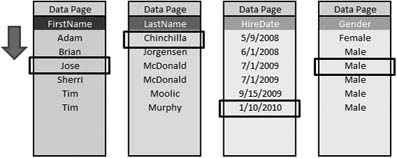
\includegraphics[width=9cm]{./Imagenes/5}
\end{center}	

%-----------------------------------------------------------------
\section{Discusión y Conclusiones}\label{sec:5}
	\begin{itemize}
		\item NoSQL permite el manejo de grandes volúmenes de datos y la posibilidad de tener un sistema distribuido.
		\item La selección de la tecnología de almacenamiento adecuada involucra la consideración de numerosos aspectos.
\item Una de las aplicaciones de la teoría de grafos se aplica en el almacenamiento de grandes cantidades de información, como por ejemplo la almacenada en una red social. 
\item Cada vez con más frecuencia estamos viendo cómo las tecnologías NoSQL forman parte de la solución en proyectos empresariales, gracias a beneficios como la mejora en la productividad de los equipos de desarrollo, y la posibilidad de llegar antes al mercado y con una considerable reducción del TCO.
	\end{itemize}


% Bibliografia.
%-----------------------------------------------------------------

\textbf{Bibliografia}\\
https://www.uaeh.edu.mx/docencia/Tesis/icbi/maestria/documentos/Consultas\\       
http://repositorio.espam.edu.ec/bitstream/42000/74/1/TESIS\\
http://repositorio.ug.edu.ec/bitstream/redug/24100/1/B-CISC-PTG.1382.Balladares \\
https://www.paradigmadigital.com/techbiz/breve-introduccion-las-tecnologias-nosql/ \\
https://smarterworkspaces.kyocera.es/blog/las-bases-datos-documentales/ \\
https://www.javeriana.edu.co/biblos/tesis/ciencias/tesis572.pdf \\


\end{document}
